
%(BEGIN_QUESTION)
% Copyright 2010, Tony R. Kuphaldt, released under the Creative Commons Attribution License (v 1.0)
% This means you may do almost anything with this work of mine, so long as you give me proper credit

Sketch connecting wires to allow this data acquisition unit (DAQ) to sense strain using quarter-bridge strain gauge circuits on input channels \#0 and \#3, such that increasing tension on the strain gauge (increasing gauge resistance) generates a more {\it positive} signal voltage on each channel:

$$\includegraphics[width=15.5cm]{i04585x01.eps}$$

\underbar{file i04585}
%(END_QUESTION)





%(BEGIN_ANSWER)

$$\includegraphics[width=15.5cm]{i04585x02.eps}$$

Challenge yourself by designing a different circuit to meet the same criteria! 

%(END_ANSWER)





%(BEGIN_NOTES)


%INDEX% Pictorial circuit review (analog signal wiring to data acquisition unit)

%(END_NOTES)

